% *********************************************************************
% © 2010–2023 Jeremy Sylvestre
%
% Permission is granted to copy, distribute and/or modify this document
% under the terms of the GNU Free Documentation License, Version 1.3 or
% any later version published by the Free Software Foundation; with no
% Invariant Sections, no Front-Cover Texts, and no Back-Cover Texts. A
% copy of the license is included in the appendix entitled “GNU Free
% Documentation License” that appears in the output document of this
% PreTeXt source code. All trademarks™ are the registered® marks of
% their respective owners.
%
% *********************************************************************

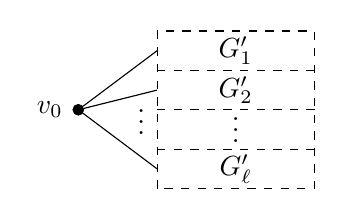
\begin{tikzpicture}[
	vertex/.style={ circle, draw, very thin, fill, inner sep=0pt, minimum size=4pt },
	vertexg/.style={ black!40!white, circle, draw, very thin, fill, inner sep=0pt, minimum size=4pt },
	vertexo/.style={ circle, draw, very thin, inner sep=0pt, minimum size=4pt }
]

\node at (0,0) (v) [vertex,label=left:$v_0$] {};
%\node at (2,0) (g) {$G'$};
\draw[dashed] (1,-1) rectangle (3,1);
\node at (2,0.75) (g1) {$G_1'$};
\draw (v) to (1,0.75);
\draw[dashed] (1,0.5) to (3,0.5);
\node at (2,0.25) (g1) {$G_2'$};
\draw (v) to (1,0.25);
\draw[dashed] (1,0) to (3,0);
\node at (2,-0.15) (g1) {$\vdots$};
\node at (0.8,-0.05) {$\vdots$};
\draw[dashed] (1,-0.5) to (3,-0.5);
\node at (2,-0.75) (g1) {$G_\ell'$};
\draw (v) to (1,-0.75);

\end{tikzpicture}
